\documentclass[../../thesis]{subfiles}
\begin{document}

\section{Scenarios}
\begin{enumerate}
    \item \emph{The validation result is logically linked to the labels/regression variable.} Given a supervised task the data $D$ is a set $\{x_i,y_i\}_i$.
    Now $\{x_i\}_i$ is constrained with the Shape Network $S_j$. Therefore there is for each $i$ a validation result $v_{i,j} \in \{0,1\}$. The model used to approximate $f$ (the real mapping $x_i \to y_i$) by $f'$ can now be further constraint given $v_{ij}$. For example there might be a logical expression stating that $\forall i ~ v_{i,2} \land ((y_i == A) \lor (y_i == B))$. 
    Given that there are multiple Shape Networks $S_j$ all associated with logical expressions, which in turn will limit the outcome of $f'(x_i)$ to some better explainable results $y_i$. 
    \begin{itemize}
        \item Are these logical expressions necessary or can they be integrated into the validation process by including the $y_i$ into the validation process?
    \end{itemize}
    
    \item \emph{The validation results are only used to limit the training data of the model to valid instances} As above $D = \{x_i, y_i\}_i$ given $S_j$ there are validation results $v_{i,j}$. But now given that there are only valid instances for training, the model can focus on learning a valid mapping $f'$. (Maybe this mapping can be made more explainable by indicating decisions which are forced by the validation process)
    
    \item \emph{Use the validation result as a further feature}
\end{enumerate}

\section{General Ideas} 
\begin{itemize}
    \item How do instances $x_i$ and knowledge graphs (including more than one instance $x_i$) interact? And how can they be separated from each other? A instances $x_i$ might be defined in terms of a query result (binding).
    \item The valid input space is constrained by the shape network.
    \item Leave out invalid instances:
    \begin{itemize}
        \item Might lead to bad generalization
        \item But the model might be more focused on the important instances
        \item Eliminates “outliers/invalid instances” → This however allows the use of models which are more sensitive to outliers
    \end{itemize}
    \item Include invalid instances but maybe remove parts of the instance which invalidates the instance (some information might be better than no information)
    \item Somehow extend the Model to support valid and invalid instances for better generalization. (see scenario 1 above)
    \item Take into account the validation result as a further parameter? 
    \item If there is some kind of a loss/cost function invalid instances could be weighted lower.
\end{itemize}


\begin{figure}[H]
    \centering
    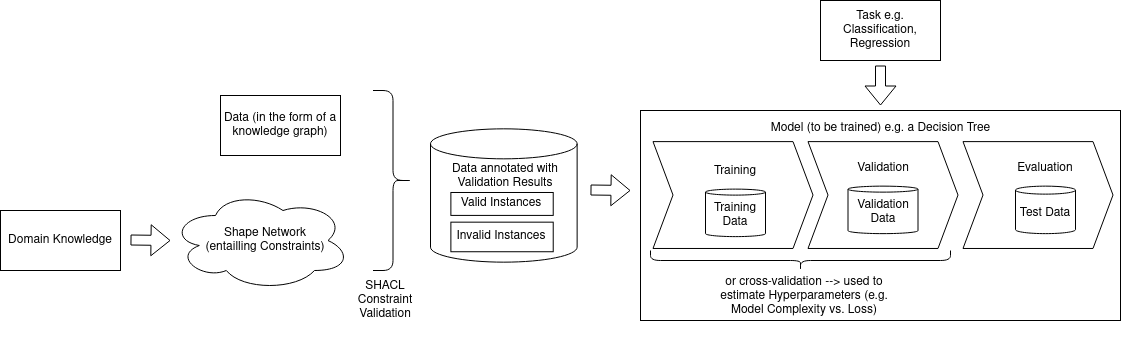
\includegraphics[width=\textwidth]{images/Supervised Pipe.png}
    \caption{Supervised Pipeline}
\end{figure}

\section{Decision Trees}



\subsection{Extension}
\begin{itemize}
    \item A path leading to a leaf/node results in a conjunction of constraints/rule of the input variables.
    \item In case of a leaf there is also an prediction → Depending on the shape network such easy constraints can be checked valid. (Presburger Arithmetic is decidable (also efficient in case of only one block of quantifiers))
    \item In most cases the Decision Tree is built completely and pruned afterwards by weighting error against model complexity. This process could be supported by considering constraints e.g. cutting of irrelevant portions of the decision tree.
    \item The “cut-off” criterion could also be modified w.r.t. invalid and valid space to suppress constraints leading to partitions only including invalid instances.
    \item Harden / Soften border constraints $\rightarrow$ Also additional constraints could be added $\rightarrow$ better understanding of the decision tree.
\end{itemize}

\section{Research Questions}
\begin{enumerate}
    \item To what extend can models be made more explainable by considering Semantic Constraint Validation?
    \item Which impact have rules/constraints on the data with respect to the time the model takes to generalize?
    \item Do the models get more accurate for example in terms of accuracy if we constraint the instances?
\end{enumerate}

\newpage

\subsection{Table of Content - Draft}
\begin{enumerate}
    \item Introduction/Motivation (Why is Explainable AI important and how can Semantic Constraint Validation be exploited to help) $\rightarrow$ Research Questions
    \item Fundamentals/Notations/Background
    \begin{enumerate}
        \item Semantic Constraint Validation
        \begin{enumerate}
            \item RDF - Knowledge Graphs
            \item SHACL - Representation of Constraints
        \end{enumerate}
        \item Machine Learning Models (Formal Definition / Applications)
        \begin{enumerate}
            \item Decision Trees, the Classification Task Definition and Regularization
            \item Random Forests - An Ensemble Learning Approach to decision trees
            \item ...
        \end{enumerate}
        \item Explainable AI $\rightarrow$ How to measure explainability?
        \item Maybe more AI Basics? Supervised Learning Learning Task / Generalization (Bias Variance Trade off) $\rightarrow$ Train/Validation/Test Split / Hyperparameters
    \end{enumerate}
    \item Extending Decision Trees
    \begin{enumerate}
        \item Formal Extension
        \item Implementation / Proof of Concept
        \item Evaluation
    \end{enumerate}
    \item Extending ...
    \item Summary
\end{enumerate}


\end{document}